%! Author = federico
%! Date = 20/01/2021

\appendix


\section{Source Code Heat Balance Model}\label{sec:python_code}

\lstinputlisting[language=Python, caption={Python code used to calculate heat losses and physiological variables as a function of environmental and personal factors},label={lst:pythonCode}, mathescape=true]{../../code/heat_balance_model.py}


\section{Validation methodology to calculate relative humidity}\label{sec:validation_rh}

In this section we present the results obtained with the following methods: the \textit{constant humidity ratio} presented in Section~\ref{subsec:weather-data}, and the \textit{coincident extreme conditions}.

\textit{Coincident extreme conditions} -- We estimated the value of \ac{rh} using the maximum extreme \ac{t-db} and \ac{t-wb} reported in the ASHRAE climate design dataset for each location.
This method assumes that both temperatures would occur at the same time in each location.
This is an approximation and it is arguably overestimating the most extreme condition because the likelihood of both conditions occurring at the same time is extremely low.

We compared the results, obtained using the aforementioned models, to the data that \mycite{Hospers2020} reported in their manuscript.
\mycite{Hospers2020} obtained hourly data for the 100 most populous metropolitan areas in the U.S.\ from January 1st, 2000 to December 31st, 2019.
They purchased the data from CustomWeather (CustomWeather, Inc., 271Miller Avenue, Mill Valley, CA, USA 94941).
From this dataset they determined the peak \ac{t-db} and corresponding \ac{rh} for each location.

Figure~\ref{fig:scatter_comparison_prediction} shows the \ac{rh} values estimated using both models and the experimental data.
The vertical error 0.7 (0.3, 1.0)~$^{\circ}$C [mean, (Q1, Q3)] is caused by the fact that \mycite{Hospers2020} data were include more recent weather observations than the ASHRAE dataset.
The horizontal error is the difference between the experimental \ac{rh} value and the one predicted by the respective model.

\begin{figure}[h]
    \centering
    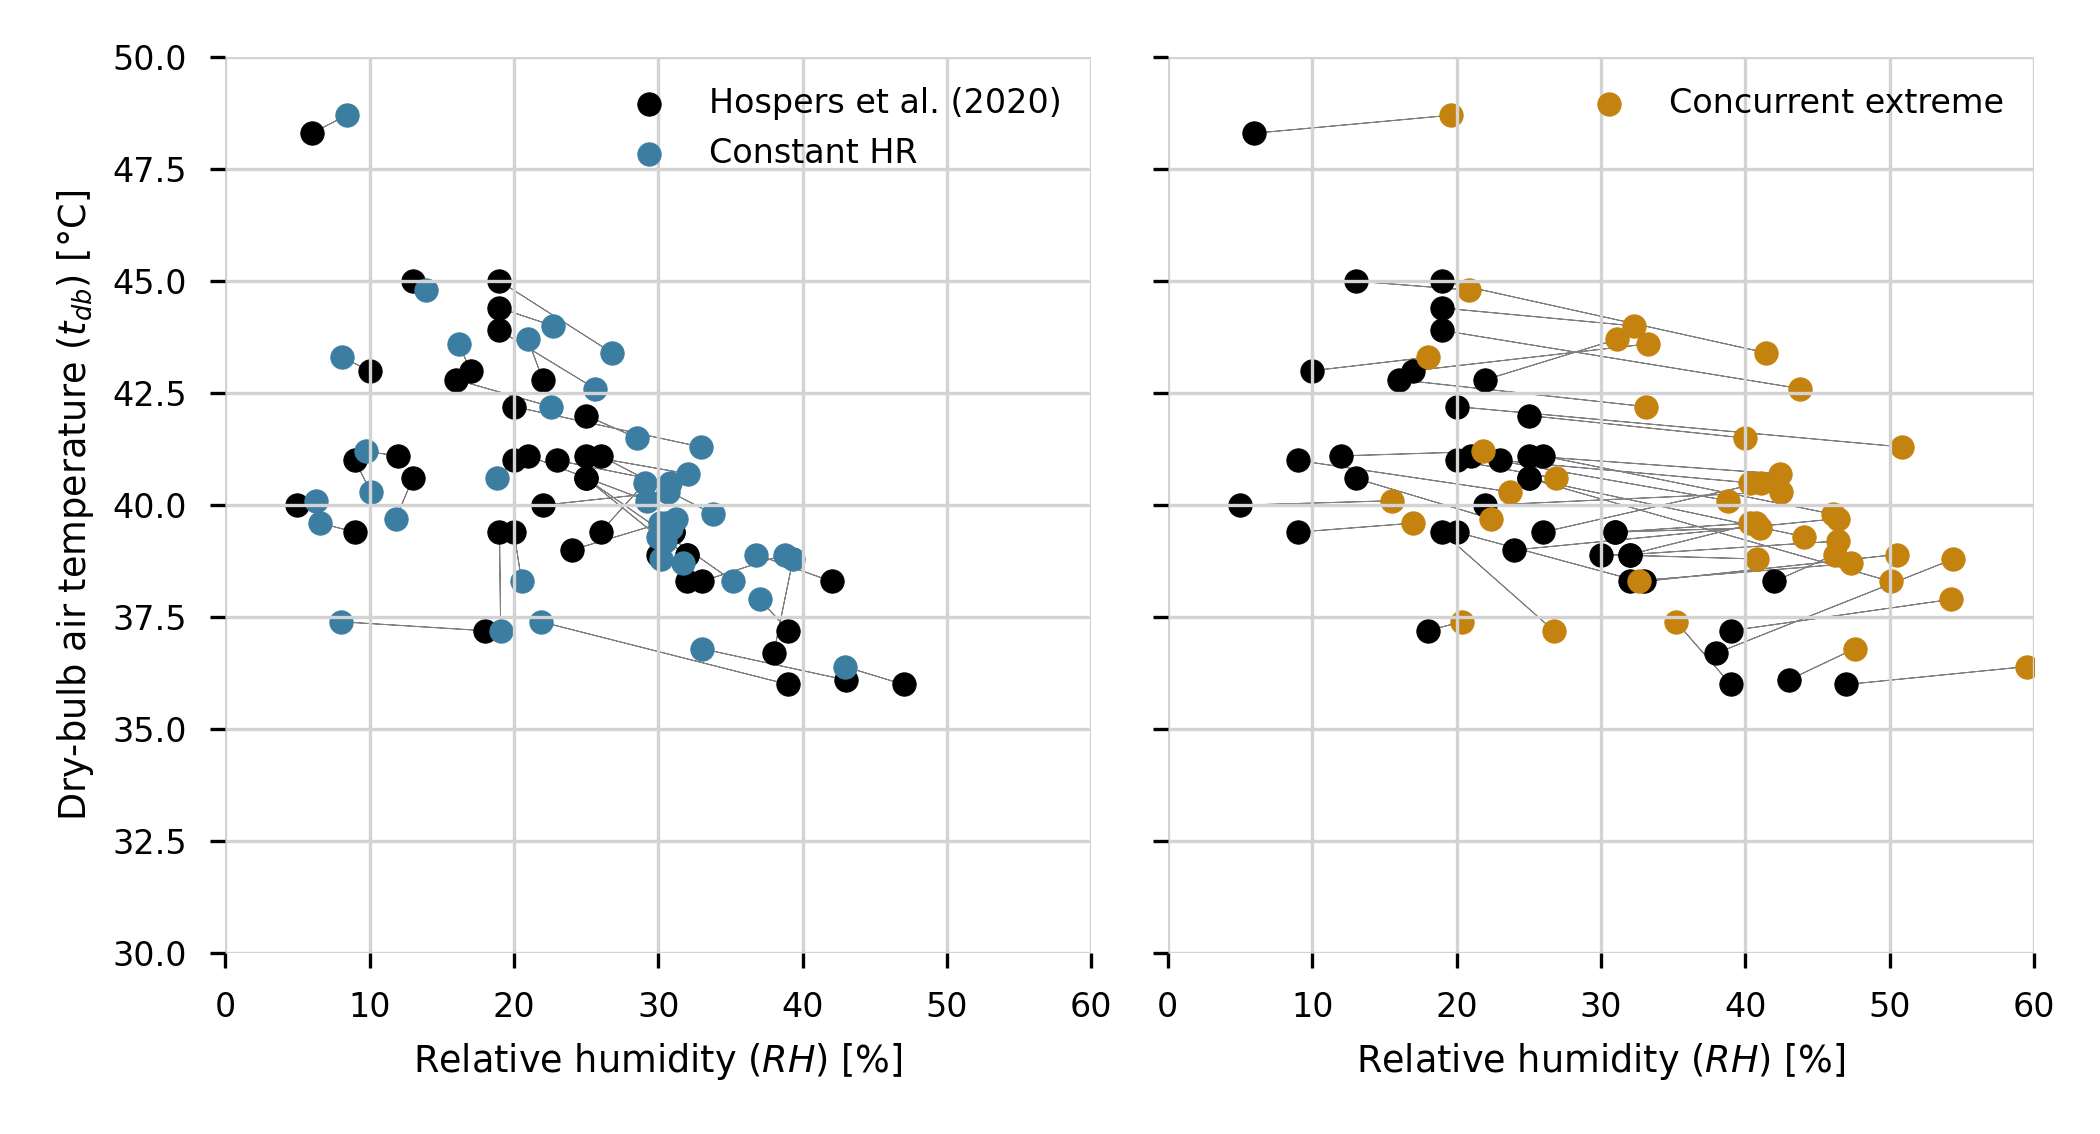
\includegraphics[width=\textwidth]{figures/scatter_comparison_prediction}
    \caption{\ac{rh} values estimated using the \textit{constant humidity ratio} and the \textit{coincident extreme conditions} models, and the experimental data from \mycite{Hospers2020}.}
    \label{fig:scatter_comparison_prediction}
\end{figure}

Figure~\ref{fig:delta_rh} shows the difference between the predicted \ac{rh} values estimated using the \textit{constant humidity ratio} and the \textit{coincident extreme conditions} models, and the experimental data from \mycite{Hospers2020}.
The predictions obtained using the \textit{constant humidity ratio} model 1.3 (-1.4, 6.3)~\% were significantly more accurate than the results obtained the \textit{coincident extreme conditions} model 13.6 (-3.8, 17.4)~\%.
The latter in the great majority of the cases overestimated the value of \ac{rh}.

\begin{figure}[h]
    \centering
    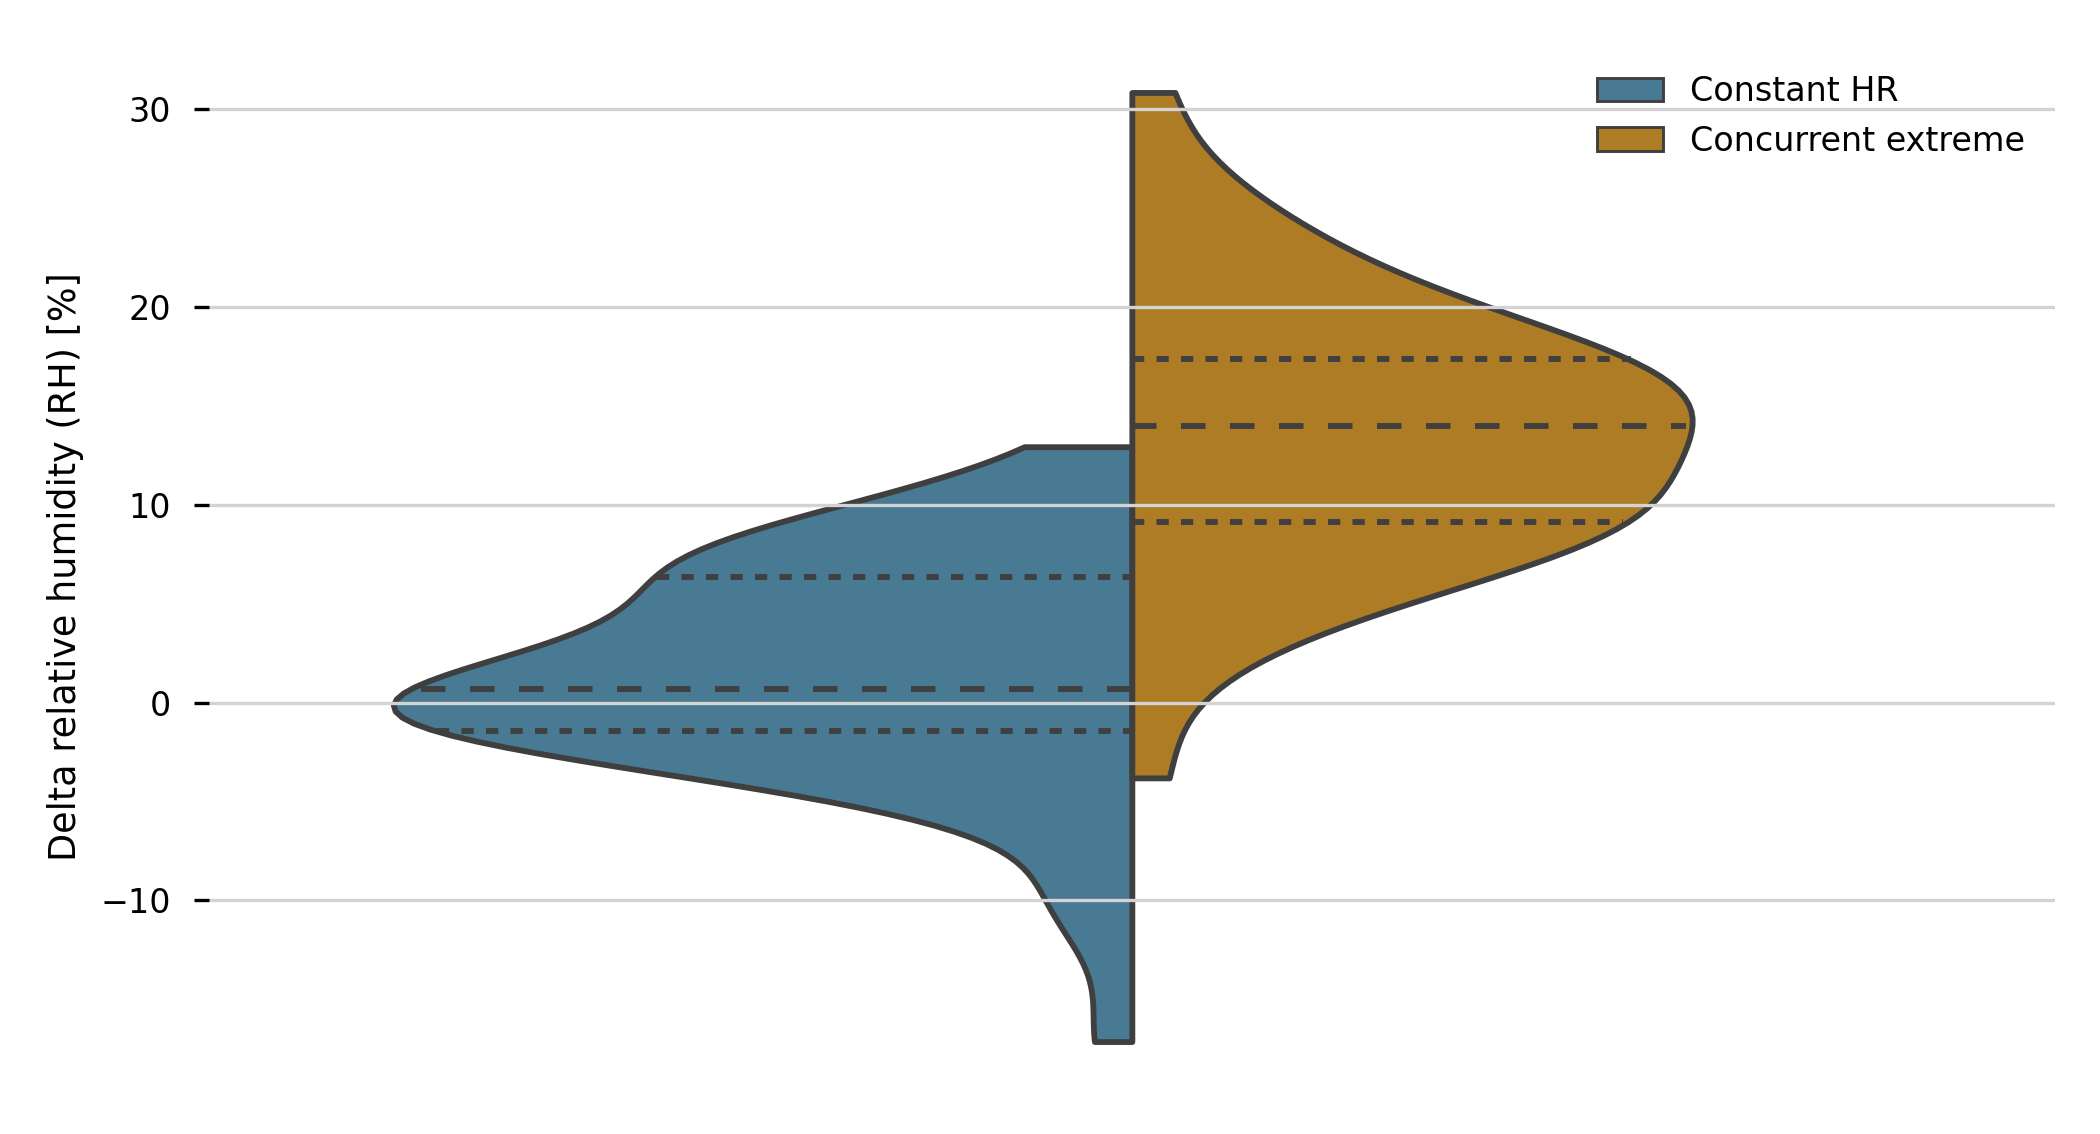
\includegraphics[width=0.5\textwidth]{figures/delta_rh}
    \caption{Difference between the predicted \ac{rh} value estimated using the \textit{constant humidity ratio} and the \textit{coincident extreme conditions}, and the experimental data from \mycite{Hospers2020}.}
    \label{fig:delta_rh}
\end{figure}

\section{Population and Weather Data}\label{sec:pop_weather}

\begin{center}
    \tiny
    \begin{longtable}{clllcc}
        \caption{Population data and maximum extreme \acf{t-db}, and \acf{t-wb} with a 20 year return period for the 115 most populous cities in the world.}
        \label{tab:pop_weather} \\

        \hline \multicolumn{1}{c}{\textbf{Rank}} & \multicolumn{1}{c}{\textbf{Country}} & \multicolumn{1}{c}{\textbf{City}}
        & \multicolumn{1}{c}{\textbf{Population}}
        & \multicolumn{1}{c}{\textbf{$t_{db}$}}
        & \multicolumn{1}{c}{\textbf{$t_{wb}$}}
        \\ \hline
        \endfirsthead

        \multicolumn{6}{c}%
        {{\bfseries \tablename\ \thetable{} -- continued from previous page}} \\
        \hline \multicolumn{1}{c}{\textbf{Rank}} & \multicolumn{1}{c}{\textbf{Country}} & \multicolumn{1}{c}{\textbf{City}}
        & \multicolumn{1}{c}{\textbf{Population}}
        & \multicolumn{1}{c}{\textbf{$t_{db}$}}
        & \multicolumn{1}{c}{\textbf{$t_{wb}$}}
        \\ \hline
        \endhead

        \hline \multicolumn{6}{r}{{Continued on next page}} \\ \hline
        \endfoot

        \hline
        \endlastfoot
   1 &               China &        Shanghai &   23019196 &     40.1 &     31.0 \\
   2 &              Mexico &          Mexico &   21942666 &     33.7 &     20.3 \\
   3 &               China &         Beijing &   19612368 &     41.6 &     30.9 \\
   4 &                U.S. &        New york &   17799861 &     39.5 &     27.7 \\
   5 &               India &          Mumbai &   16434386 &     41.4 &     30.0 \\
   6 &           Argentina &    Buenos aires &   15416728 &     38.4 &     28.8 \\
   7 &            Pakistan &         Karachi &   14910352 &     44.4 &     31.7 \\
   8 &               India &           Delhi &   12877470 &     48.3 &     32.5 \\
   9 &               Japan &           Tokyo &   12576601 &     37.6 &     29.2 \\
  10 &                U.S. &     Los angeles &   11789487 &     37.9 &     24.0 \\
  11 &  Russian federation &          Moskva &   11503501 &     36.3 &     24.5 \\
  12 &              Brazil &       Sao paulo &   11152968 &     36.2 &     27.2 \\
  13 &            Pakistan &          Lahore &   11126285 &     47.1 &     31.5 \\
  14 &              France &           Paris &   10706072 &     38.5 &     25.0 \\
  15 &         South korea &           Seoul &    9704546 &     37.1 &     28.8 \\
  16 &               China &       Chongqing &    9691901 &     42.3 &     30.2 \\
  17 &           Indonesia &         Jakarta &    9607787 &     36.8 &     31.9 \\
  18 &                Peru &            Lima &    9562280 &     32.4 &     25.3 \\
  19 &               Egypt &           Cairo &    9539673 &     45.1 &     28.0 \\
  20 &                Iran &          Tehran &    8693706 &     42.8 &     25.3 \\
  21 &               China &       Guangzhou &    8524826 &     39.7 &     29.4 \\
  22 &               China &           Wuhan &    8312700 &     40.1 &     32.1 \\
  23 &                U.S. &         Chicago &    8307904 &     39.6 &     27.6 \\
  24 &            Thailand &         Bangkok &    8305218 &     40.5 &     32.7 \\
  25 &      United kingdom &          London &    8278251 &     35.8 &     22.6 \\
  26 &           Hong kong &   Hong kong sar &    7507400 &     34.1 &     28.4 \\
  27 &               China &         Tianjin &    7499181 &     40.0 &     30.1 \\
  28 &               China &        Shenzhen &    7008831 &     38.1 &     31.1 \\
  29 &            Colombia &          Bogota &    6778691 &     27.6 &     23.0 \\
  30 &              Canada &         Toronto &    6471850 &     37.9 &     28.9 \\
  31 &              Brazil &  Rio de janeiro &    6320446 &     39.0 &     28.9 \\
  32 &               India &       Hyderabad &    5742036 &     44.8 &     29.6 \\
  33 &           Singapore &       Singapore &    5703569 &     35.8 &     29.2 \\
  34 &               India &       Bangalore &    5701446 &     37.7 &     28.6 \\
  35 &               India &       Ahmadabad &    5633927 &     46.8 &     32.8 \\
  36 &               Chile &        Santiago &    5428590 &     36.2 &     22.2 \\
  37 &               China &        Shenyang &    5303053 &     35.7 &     28.6 \\
  38 &              Mexico &     Guadalajara &    5243178 &     37.7 &     23.5 \\
  39 &             Myanmar &          Yangon &    5211431 &     41.4 &     31.7 \\
  40 &        Saudi arabia &          Riyadh &    5188286 &     47.8 &     25.3 \\
  41 &               Egypt &      Alexandria &    5163750 &     43.1 &     28.7 \\
  42 &                U.S. &    Philadelphia &    5149079 &     39.7 &     29.2 \\
  43 &              Mexico &       Monterrey &    5133917 &     45.1 &     31.6 \\
  44 &                U.S. &           Miami &    4919036 &     38.8 &     30.3 \\
  45 &  Russian federation &  St. petersburg &    4879566 &     35.7 &     25.5 \\
  46 &           Australia &          Sydney &    4835206 &     45.0 &     25.7 \\
  47 &           Australia &       Melbourne &    4784608 &     44.3 &     25.2 \\
  48 &               India &         Chennai &    4646732 &     44.4 &     31.2 \\
  49 &               India &           Surat &    4501610 &     43.2 &     30.0 \\
  50 &               India &         Kolkata &    4496694 &     42.9 &     32.2 \\
  51 &               China &           Xi'an &    4481508 &     41.3 &     26.2 \\
  52 &               Kenya &         Nairobi &    4397073 &     34.4 &     22.3 \\
  53 &       Cote d'ivoire &         Abidjan &    4395243 &     38.7 &     31.0 \\
  54 &               China &         Chengdu &    4333541 &     38.4 &     30.3 \\
  55 &              Canada &        Montreal &    4318505 &     35.5 &     27.8 \\
  56 &                U.S. &          Dallas &    4145659 &     43.7 &     28.1 \\
  57 &                U.S. &          Boston &    4032484 &     38.8 &     27.1 \\
  58 &              Jordan &           Amman &    4007526 &     42.9 &     25.7 \\
  59 &               Spain &          Madrid &    3998829 &     41.0 &     25.3 \\
  60 &                U.S. &      Washington &    3933920 &     47.7 &     31.4 \\
  61 &                U.S. &         Detroit &    3903377 &     38.7 &     28.6 \\
  62 &                Iraq &         Baghdad &    3841268 &     51.0 &     27.0 \\
  63 &                U.S. &         Houston &    3822509 &     41.3 &     31.6 \\
  64 &               Japan &        Yokohama &    3724844 &     36.7 &     28.3 \\
  65 &               China &         Nanjing &    3624234 &     39.7 &     30.8 \\
  66 &             Germany &          Berlin &    3613495 &     39.3 &     23.5 \\
  67 &                U.S. &         Atlanta &    3499840 &     39.3 &     28.3 \\
  68 &               China &         Haerbin &    3481504 &     37.7 &     27.1 \\
  69 &        Saudi arabia &          Jiddah &    3430697 &     49.4 &     34.6 \\
  70 &         South korea &           Busan &    3400027 &     35.0 &     29.3 \\
  71 &               China &          Dalian &    3245191 &     36.9 &     29.5 \\
  72 &               China &       Changchun &    3225557 &     36.7 &     27.4 \\
  73 &              Mexico &          Puebla &    3179162 &     32.7 &     22.7 \\
  74 &               India &            Pune &    3124458 &     41.9 &     28.8 \\
  75 &               India &          Jaipur &    3046163 &     47.0 &     31.5 \\
  76 &               China &         Kunming &    3035406 &     32.1 &     23.4 \\
  77 &                Iran &         Mashhad &    3001184 &     42.5 &     25.6 \\
  78 &               China &           Jinan &    2999934 &     40.4 &     29.8 \\
  79 &                U.S. &   San francisco &    2995769 &     37.2 &     22.2 \\
  80 &               China &         Guiyang &    2985105 &     35.4 &     26.3 \\
  81 &         South korea &         Incheon &    2938875 &     35.8 &     29.3 \\
  82 &         Philippines &     Quezon city &    2936116 &     39.2 &     32.5 \\
  83 &                U.S. &         Phoenix &    2907049 &     48.7 &     27.4 \\
  84 &             Ukraine &            Kyiv &    2893215 &     38.1 &     25.0 \\
  85 &               Italy &            Roma &    2864466 &     39.4 &     28.4 \\
  86 &               India &         Lucknow &    2817105 &     46.8 &     32.7 \\
  87 &               India &          Kanpur &    2768057 &     46.8 &     32.7 \\
  88 &           Indonesia &        Surabaya &    2765487 &     36.7 &     30.5 \\
  89 &               China &         Qingdao &    2720972 &     39.2 &     29.7 \\
  90 &             Algeria &         Algiers &    2712944 &     45.0 &     29.1 \\
  91 &                U.S. &         Seattle &    2712205 &     38.3 &     24.6 \\
  92 &              Canada &       Vancouver &    2691351 &     31.7 &     22.8 \\
  93 &               Japan &           Osaka &    2691185 &     39.6 &     28.6 \\
  94 &              Brazil &        Salvador &    2674923 &     37.7 &     30.6 \\
  95 &                U.S. &       San diego &    2674436 &     37.4 &     24.6 \\
  96 &             Hungary &        Budapest &    2608485 &     39.1 &     25.1 \\
  97 &               China &       Zhengzhou &    2589387 &     41.5 &     31.0 \\
  98 &         North korea &       Pyongyang &    2581076 &     35.4 &     28.9 \\
  99 &               China &         Taiyuan &    2558382 &     39.3 &     28.4 \\
 100 &          Uzbekistan &        Tashkent &    2509969 &     44.1 &     27.4 \\
 101 &              Brazil &        Brasilia &    2481272 &     36.0 &     26.6 \\
 102 &               China &        Chaoyang &    2470812 &     41.0 &     28.4 \\
 103 &              Brazil &       Fortaleza &    2452185 &     35.4 &     30.5 \\
 104 &               China &        Hangzhou &    2451319 &     40.5 &     30.3 \\
 105 &         South korea &           Daegu &    2449789 &     38.5 &     28.0 \\
 106 &               India &          Nagpur &    2405665 &     48.7 &     32.0 \\
 107 &                U.S. &     Minneapolis &    2388593 &     39.2 &     28.8 \\
 108 &           Australia &        Brisbane &    2379724 &     42.1 &     27.8 \\
 109 &              Mexico &          Toluca &    2377828 &     30.8 &     19.4 \\
 110 &              Brazil &  Belo horizonte &    2375151 &     36.8 &     27.3 \\
 111 &               Japan &          Nagoya &    2295638 &     39.6 &     28.5 \\
 112 &             Ecuador &       Guayaquil &    2278738 &     36.0 &     27.9 \\
 113 &          Azerbaijan &            Baku &    2270030 &     40.0 &     31.6 \\
 114 &      United kingdom &      Manchester &    2244931 &     32.6 &     22.3 \\
 115 &               China &        Changsha &    2122873 &     40.1 &     30.2 \\
    \end{longtable}
\end{center}


\begin{figure*}[hbt!]
    \centering
    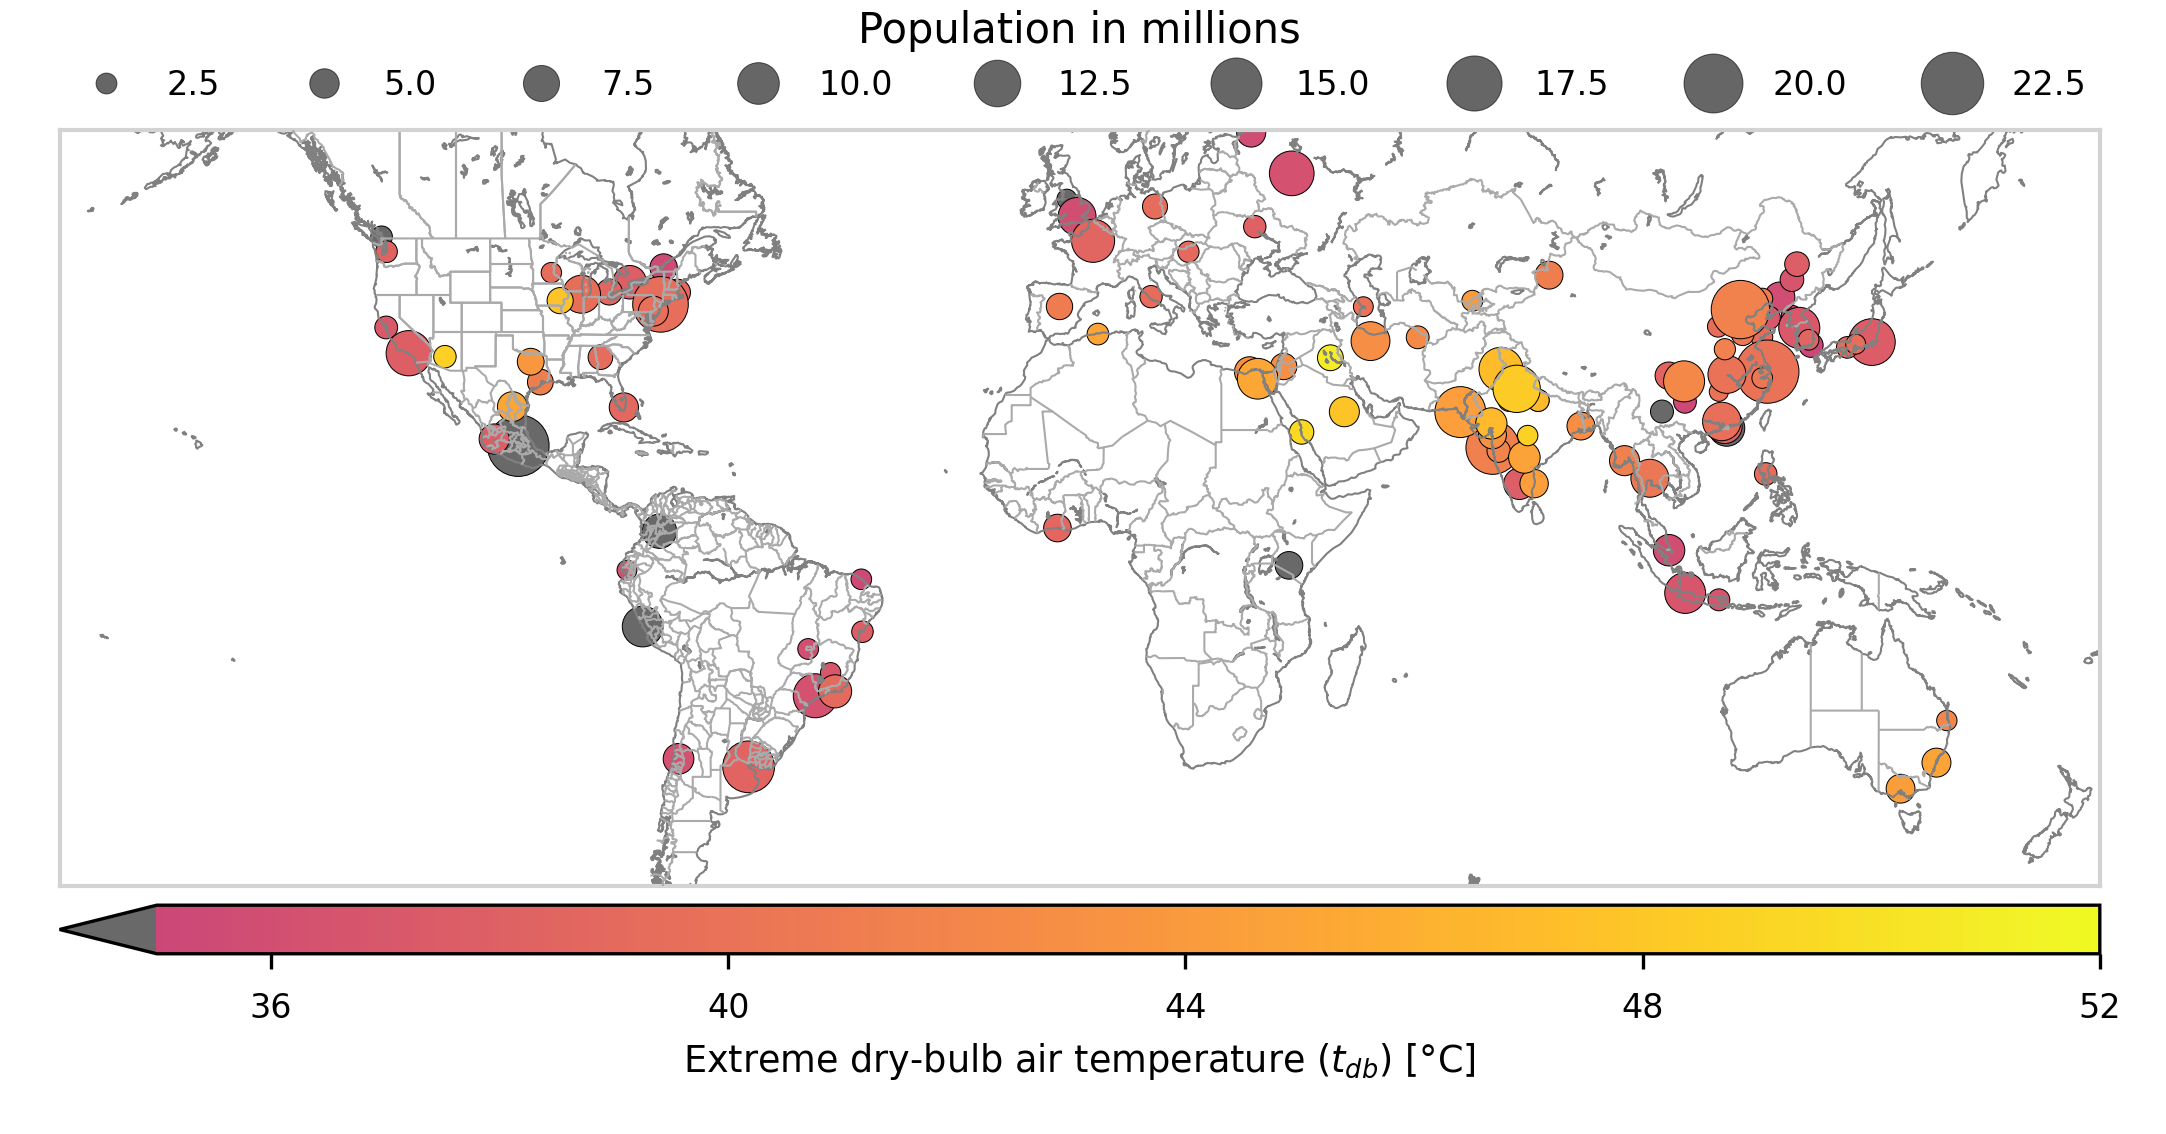
\includegraphics[width=\textwidth]{figures/map-population-temperature}
    \caption{Most populous 115 cities worldwide}
    \label{fig:map-population-temperature}
\end{figure*}

\begin{figure*}[hbt!]
    \centering
    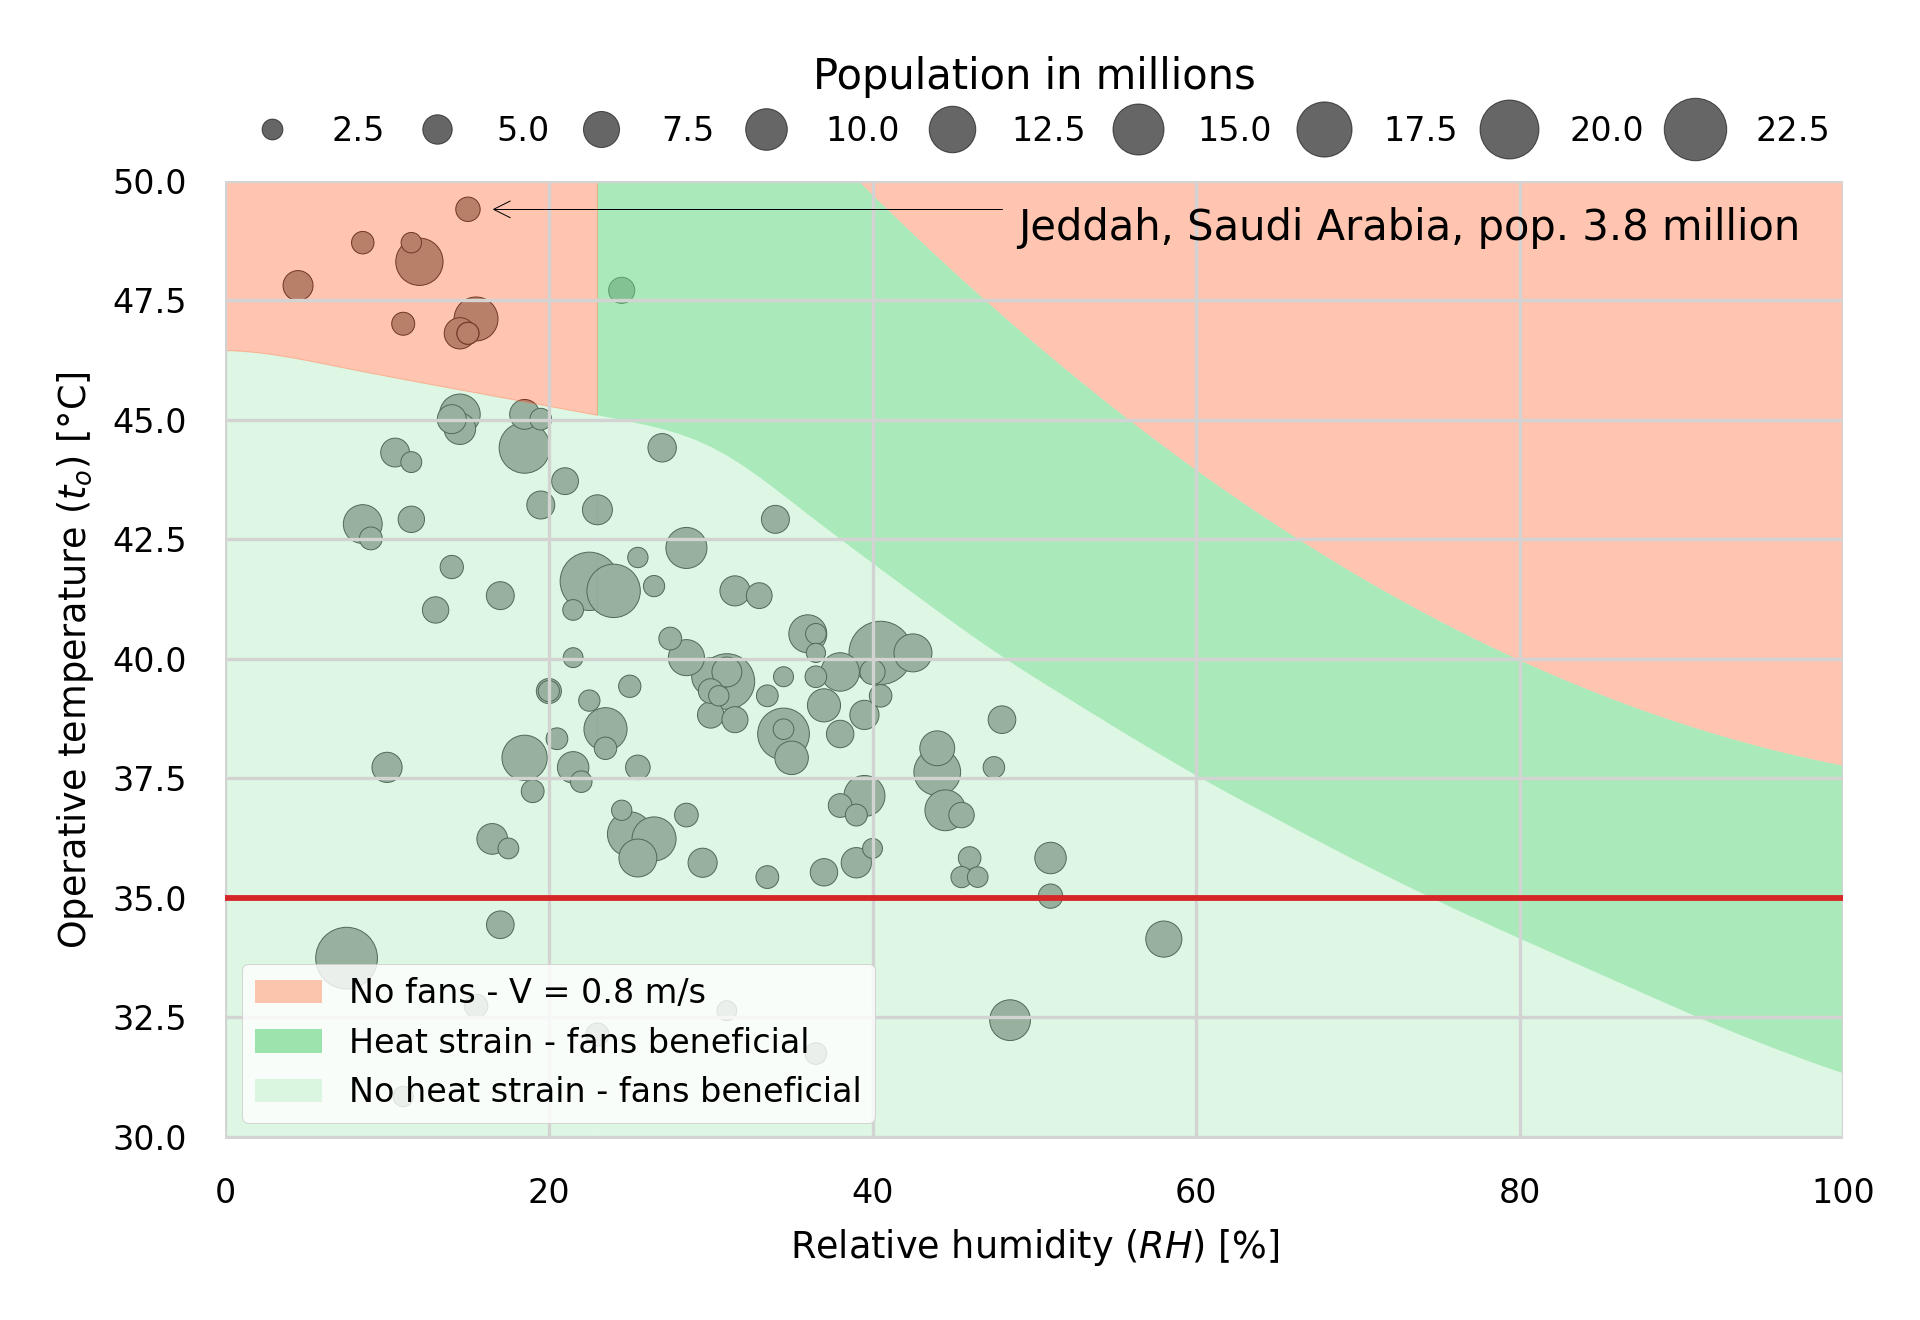
\includegraphics[width=\textwidth]{figures/use_fans_and_population}
    \caption{Environmental conditions under which the use of electric fans is beneficial, for more information on how to interpret the Figure please refer to the caption of Figure~\ref{fig:use_fans_experimental}.
    Each dot shows the maximum extreme climate conditions recorded over the last 20 years in each of the 115 most populous cities worldwide.}
    \label{fig:use_fans_and_population}
\end{figure*}

\clearpage